\section{Cache Coherence Timing Channel}
In a multi-core system, threads are running concurrently on different cores. These threads may share some
data which they read from or write to. The shared data thus can have multiple copies exist in each core's
private cache. In general, a cache coherence protocol is used to ensure each thread gets the most updated
data to work with.

In a snooping-based protocol, the caches on the same level are connected with a snooping bus. When a request
comes into a cache and incurs a cache miss, a snooping request is sent on the snooping bus. All the other
caches observe the snooping request, and one of them may respond to the request by forwarding the data if 
the data exists. The operations to handle snooping requests and responses highly depend on the specific cache 
coherence protocols being used. Commonly used protocols include MSI, MESI and MOESI~\cite{mark_book}.

If different timing compartments share data, there is clearly a timing channel introduced by the cache coherence
protocols. For example, TC0 wants to write to A, and A exists in TC1's cache. In order to perform the write, the
cache coherence protocol will invalidate A in TC1's cache. Later when TC1 wants to read A, it will incur a cache
miss which indicates TC0 has written to A. In our threat model, we assume timing compartments do not share data. 
So the above mentioned timing channel is not a concern. However, our assumption only guarantees the cache state
is not affected by cache coherence protocols. The snooping bus is shared by different timing compartments, thus 
the coherent traffic can still interfere with each other. The interference on the snooping bus introduces timing
channel, as shown in the example below.

\subsection{Covert Channel Attack Example}
In this section, we demonstrate a covert channel attack example on a four-core system. The system configuration 
is shown in Figure~\ref{fig:coherent_system}. Each core has a private L1 and L2 cache, and the four cores share
the L3 cache. The four L2 caches are connected with a snooping bus which uses a MOESI protocol. 
In this example, there are two attackers who
want to communicate a secret data when the direct communication between them is strictly disallowed. Each attacker 
belongs to a different timing compartment. Attacker0 occupies core 0 and core 1 while attacker1 occupies core 2 and
core 3. 

\begin{figure}
    \begin{center}
        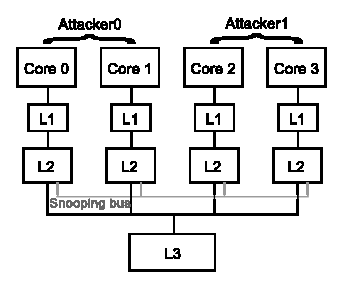
\includegraphics[width=2.3in]{figs/coherent_system.eps}
        \caption{System Configuration}
        \label{fig:coherent_system}
    \end{center}
\end{figure}

Attacker0 has two threads, each running on a different core. Both threads run a $for$ loop of 4000 iterations, and
write to a shared data in each iteration. Before each write is performed, one L2 cache has to forward the data
to the other L2 cache through the snooping bus and invalidates its own copy, according to the cache coherence protocol. 
As a result, there is a lot of coherent traffic between these two threads. Attacker0 runs this $for$ loop repeatedly and
records the time to finish the $for$ loop using c++ timing functions.

Attacker1 owns the secret data ('01101100') and tries to communicate this secret to Attacker0. It checks each bit
in the secret data. If the bit is 0, it executes a $for$ loop which writes to a data in each iteration. This does not produce 
coherent traffic. If the bit is 1, Attacker1 spawns a new thread, which also runs a $for$ loop that writes to the same data, hence producing a lot of coherent traffic. 

\begin{figure}
    \begin{center}
        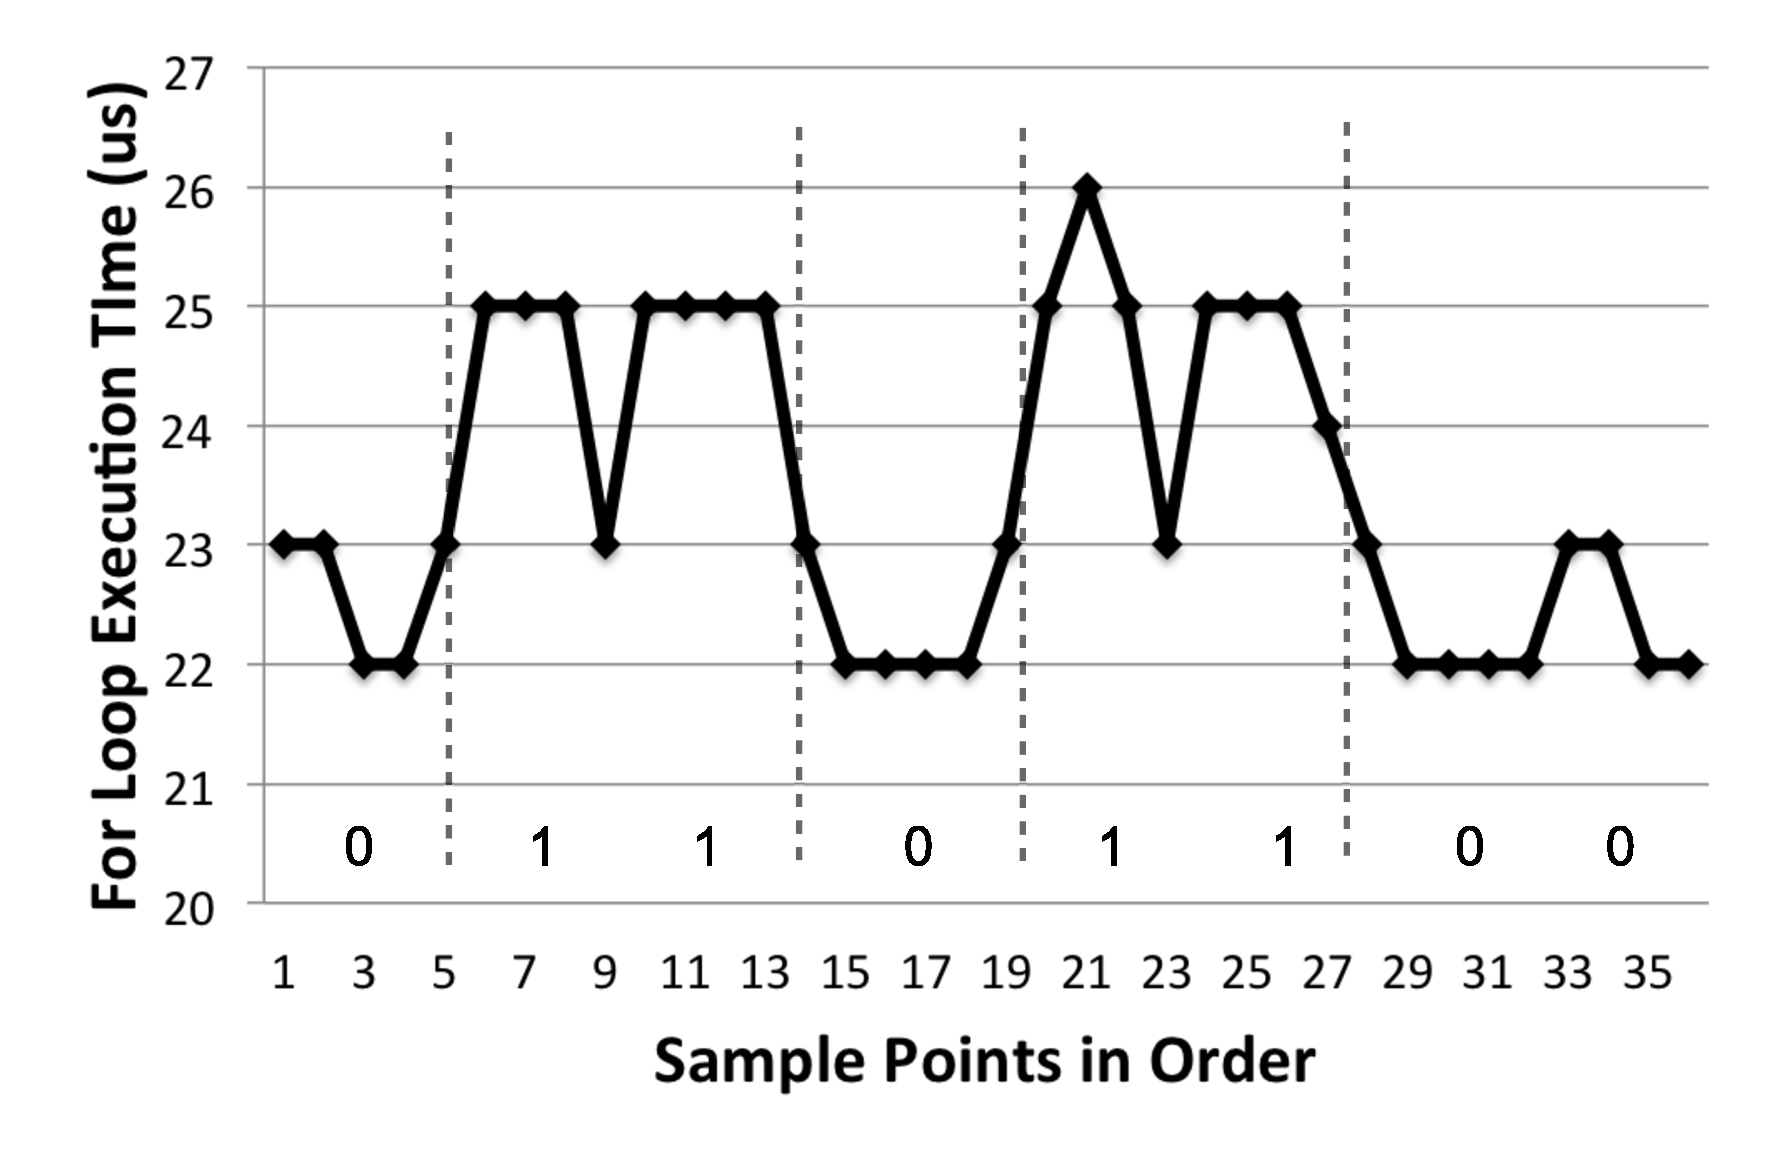
\includegraphics[width=2.79in]{figs/coherence_interference.eps}
        \caption{Attacker0's Timing Observation}
        \label{fig:coherence_interference}
    \end{center}
\end{figure}

Note that in this example, we have all the aforementioned protection schemes implemented except for the snooping bus.
Figure~\ref{fig:coherence_interference} shows the $for$ loop execution time sequence that Attacker0 observes. Each
sample point represents the time it takes to finish a 4000 iteration $for$ loop. Based on the observation, Attacker0
can recover the secret successfully. The timing variation is caused by the interference on the snooping bus. If Attacker1
produces a lot of coherent traffic, Attacker0's coherent traffic gets delayed and thus finishes slower compared to
when Attacker1 does not produce coherent traffic. 

\subsection{Protection Scheme}
The protection scheme is similar to the normal bus protection. We attached the TCID to the snooping requests and responses.
The snooping bus scheduling is changed to round-robin scheduling. With this protection, the coherent traffic from different
timing compartments do not interfere with each other through the snooping bus. This protection prevents the covert channel
attack mentioned above.
